\begin{lpu}{Wie ein Computer Fragen stellt: Entscheidungsbäume}

Das Motto von diesem Kapitel lautet: \textit{Gute Fragen führen zu guten Vorhersagen}. Sie lernen hier ein zentrales Werkzeug des maschinellen Lernens kennen: den \textbf{Entscheidungsbaum}. Ein solcher Baum ist eine strukturierte Darstellung von Regeln, mit denen sich Vorhersagen treffen lassen. Doch bevor wir uns in die Formalitäten stürzen, starten wir mit einem Spiel — denn Maschinenlernen ist in vielen Fällen gar nicht so verschieden davon, wie Menschen lernen.

\begin{aufgabe}{1: 20 Questions}
Spielen Sie zuerst mit einem Partner\footnote{Falls Sie diese LPU nicht im Klassenverband durcharbeiten, können Sie auch \href{http://www.20q.net/}{online} (\href{http://www.20q.net/}{\url{20q.net}}) spielen} eine Runde \emph{20 Questions}:
\begin{itemize}
  \item Eine Person denkt sich ein Objekt aus.
  \item Die andere darf nur \textbf{binäre Fragen} stellen, also solche, die mit „ja“ oder „nein“ beantwortet werden können.
  \item Ziel ist es, das Objekt möglichst effizient zu erraten.
\end{itemize}

Überlegen Sie sich daraufhin Antworten auf die folgenden Punkte:
\begin{enumerate}
  \item Notieren Sie drei besonders hilfreiche Fragen, die viele Möglichkeiten auf einmal ausschliessen.
  \item Was macht diese Fragen „gut“?
  \item Formulieren Sie eine Regel: Wann ist eine Frage besonders hilfreich?
\end{enumerate}
\end{aufgabe}

Was dieses Spiel technisch betrachtet macht: 
\begin{itemize}
    \item Das ausgedachte Objekt hat mehrere Eigenschaften (= Attribute, bspw: Ein Elefant hat eine Farbe, ein Gewicht, ist ein Tier, hat einen Rüssel etc.).
    \item Wir versuchen, das Objekt einer passenden Kategorie zuzuordnen (graues, 5 Tonnen schweres Tier mit Rüssel \Rightarrow Elefant).
    \item Zur Auswahl (= mögliche Kategorien) stehen alle Wörter, die im Alltag gebräuchlich sind (Elefant, Auto, Milchstrasse, Justizsystem...).
    \item Um diese Zuordnung zu einer dieser Kategorien vorzunehmen, nehmen wir die Attribute zu Hilfe.
\end{itemize}

Wenn wir das Vorgehen so formalisieren, dann lässt sich erkennen, dass auch ein Computer ein solches Vorgehen umsetzen könnte. Für jede Kategorie müssten wir also die passenden Attribute in Form einer Regel festhalten und das ausgedachte Objekt mit diesen Regeln vergleichen. In Pseudocode könnten diese Regeln wie folgt aussehen: \noindent\colorbox{orange!10}{\texttt{X.color == "grey"\ and X.weight == 5000 and X.has\_trunk == True}}.

\begin{aufgabe}{2}
\label{sec:elephant}
Erweitern Sie die obige Regel so, dass Sie auch \textit{weisse} Tiere mit Rüssel, die zwischen 2 und 6 Tonnen wiegen, als Elefanten klassifiziert werden. Gehen Sie dabei in zwei Schritten vor:
\begin{enumerate}
    \item ``Kleben'' Sie zunächst einzelne Vergleichsausdrücke mit \texttt{or} aneinander: Aus \texttt{a == b}, zum Beispiel, wird also \texttt{a == b or a == c}
    \item Überführen Sie dann die ganze ``zusammengeklebte'' Regel in eine Form, die sich mit binären Fragen abfragen lässt. Eine Bedingung wie \texttt{(A or B) and C} können Sie nicht direkt als eine einzige Frage stellen, da sie mehr als eine Bedingung kombiniert. Stattdessen teilen Sie diese auf in zwei Fragen:
    \begin{itemize}
        \item Zuerst \texttt{A and C},
        \item dann \texttt{B and C}.
    \end{itemize}
    Zusammen entspricht dies \texttt{(A and C) or (B and C)}. Gehen Sie sinngemäss mit Ihren Bedingungen vor.
\end{enumerate}
\end{aufgabe}

Nun haben Sie eine grosse Regel, die alle Möglichkeiten abdeckt, die zu einer Klassifikation zum Elefanten führen.

\begin{hinweis}
Diese Umformung, die Sie oben vornehmen, ist ein Beispiel dafür, wozu wir die Gesetze der Bool'schen Algebra verwenden können: hier wenden Sie das Distributivgesetz an. Es erlaubt, logische Ausdrücke so umzuformen, dass sie nur noch aus einfachen \texttt{and}- und \texttt{or}-Verknüpfungen bestehen.

In der überführten Version entsteht eine Struktur, die man als \textbf{disjunktive Normalform (DNF)} bezeichnet: eine Reihe von Bedingungen, bei denen jeweils mehrere Merkmale gemeinsam zutreffen müssen (\texttt{a and c}, \texttt{b and c}), verbunden durch ein \texttt{or}. Solche Formen sind besonders hilfreich, wenn man aus komplexen Regeln konkrete binäre Fragen ableiten möchte – wie etwa im Spiel \emph{20 Questions} oder in einem Entscheidungsbaum, wie wir gleich sehen werden. Obwohl dies noch nicht zum Inhalt dieser Lerneinheit gehört, zeigt es, wie Sie Wissen aus anderen Gebieten der Informatik miteinander verknüpfen können.
\end{hinweis}

Nehmen wir nun einige neue Regeln zur Hand, um das weitere Vorgehen zu demonstrieren:

\begin{itemize}
    \item Auto: \texttt{X.has\_wheels == True and X.is\_visible == True and X.is\_man\_made == True and X.is\_institution == False}
    \item Milchstrasse: \texttt{X.has\_wheels == False and X.is\_visible == True and X.is\_man\_made == False and X.is\_institution == False}
    \item Justizsystem: \texttt{X.has\_wheels == False and X.is\_visible == False and X.is\_man\_made == True and X.is\_institution == True} 
\end{itemize}

Wenn wir mit diesen Regeln das Spiel spielen wollten, würden wir gut daran tun, nicht \textit{alle} 12 Vergleiche zu erfragen, sondern die nächste Frage abhängig von der Antwort der vorhergehenden Frage zu machen. Dazu sei Ihnen folgender Startpunkt gegeben:

\begin{center}
\begin{tikzpicture}[
  node distance=1.8cm and 2.8cm,
  every node/.style={font=\sffamily},
  decision/.style={rectangle, draw, minimum width=2.5cm, minimum height=1cm, fill=blue!10},
  leaf/.style={rectangle, draw, minimum width=2.5cm, minimum height=1cm, fill=green!10}
  ]

\node[decision] (wheels) {\texttt{X.has\_wheels}};
\node[leaf, below left=of wheels] (auto) {?};
\node[leaf, below right=of wheels] (visible) {?};

\draw[->] (wheels) -- node[left] {\texttt{True}} (auto);
\draw[->] (wheels) -- node[right] {\texttt{False}} (visible);

\end{tikzpicture}
\end{center}

\begin{aufgabe}{3}
Überführen Sie die 3 Regeln oben in ein Diagramm, sodass Sie mit \textit{weniger} als 12 Fragen ein Objekt einer der drei Kategorien zuordnen können.
\end{aufgabe}


\begin{aufgabe}{3: Zusatzaufgabe}
Erweitern Sie Ihr System so, dass es auch eine Möglichkeit gibt, ein Objekt einer \textit{Sonstiges}-Kategorie zuzuordnen.
\end{aufgabe}

Sie haben nun vermutlich gemerkt: Nicht alle Eigenschaften sind gleich nützlich. Manche Fragen schaffen sofort Klarheit („Hat es Räder?“ – dann ist es wohl ein Auto), andere schliessen nur wenig aus.

Vielleicht haben Sie sogar überlegt, in welcher Reihenfolge Fragen gestellt werden sollten, um möglichst schnell zum Ziel zu kommen. Und womöglich haben Sie gemerkt, dass sich diese Entscheidungen gut in einer Art binären Baum, wie Sie ihn bereits aus dem Informatik-Unterricht kennen organisieren lassen, bei dem man immer nur zwei Wege weiterverfolgt – je nachdem, ob die Antwort \texttt{True} oder \texttt{False} ist.

Genau solche Strukturen tauchen in der Informatik und im maschinellen Lernen häufig auf – und sie lassen sich sogar automatisiert berechnen.

\begin{theorie}
Ein \textbf{Entscheidungsbaum} im ML funktioniert genau so: Er stellt nacheinander binäre Fragen zu den Eigenschaften eines Datenpunktes mit verschiedenen Eigenschaften, um am Ende eine Entscheidung darüber zu treffen, zu welcher Kategorie dieser Datenpunkt gehört.
\end{theorie}

Sie haben also intuitiv eine der wichtigsten Strukturen des maschinellen Lernens entdeckt.


\begin{aufgabe}{4}
Öffnen Sie die beiliegende Datei \texttt{LA\_1605\_Geschlechter.xlsx}. Darin finden Sie eine Liste mit Grösse, Gewicht und Geschlecht\footnote{In dieser Liste sind alle Datenpunkte entweder \texttt{Male} oder \texttt{Female}. Das bedeutet aber nicht, dass es nicht auch Personen gibt, welche sich in diesen Kategorien nicht abgebildet sehen.} von Personen.

\begin{enumerate}
  \item Überlegen Sie sich eine einfache binäre Frage basierend auf Gewicht oder Grösse, mit der Sie versuchen, das Geschlecht vorherzusagen.
  \item Tragen Sie in einer neuen Spalte (\textit{Vorhersage des Entscheidungsbaumes} ein, ob die Regel korrekt liegt, indem Sie mit dem \textit{tatsächlichen Gewicht} vergleichen
  \item Zählen Sie: Wie oft lag Ihre Vorhersage richtig?
  \item Versuchen Sie zwei weitere Vergleiche hinzuzufügen und vergleichen Sie das Resultat.
  \item Was passiert, wenn Sie die Reihenfolge Ihrer Fragen ändern?
\end{enumerate}
\end{aufgabe}

Herzlichen Glückwunsch! Sie haben Ihren ersten Entscheidungsbaum entwickelt und dessen Qualität überprüft!

\begin{theorie}
Wie Sie gelernt haben, bestehen Entscheidungsbäume aus:
\begin{itemize}
  \item \textbf{Knoten:} eine Frage (z. B. \texttt{X.Grösse $>$ 175})
  \item \textbf{Äste:} die Antwortmöglichkeiten (\texttt{True} und \texttt{False})
  \item \textbf{Blätter:} die Kategorisierung (z. B. \texttt{männlich})
\end{itemize}
\end{theorie}

\begin{aufgabe}{5: Eintrag ins Glossar}
Formuliere in Deinen eigenen Worten eine Definition für:

\textbf{decision tree (Entscheidungsbaum):} \\
\underline{\hspace{15cm}}
\end{aufgabe}

Der in der nachfolgenden Aufgabe eingesetzten \textbf{Titanic-Datensatz} ist einer der bekanntesten und am weitesten verbreiteten Datensätze in der Welt des maschinellen Lernens. Er wird häufig in Lehrbüchern, Kursen und Einführungsvideos verwendet, weil er reale historische Daten enthält, aber dennoch klein und übersichtlich genug ist, um erste Werkzeuge wie Entscheidungsbäume daran zu erproben.

Obwohl der Datensatz aus einem tragischen historischen Ereignis stammt, wird er in der Informatik didaktisch genutzt, um grundlegende Ideen des maschinellen Lernens anschaulich zu machen – etwa wie man mit einfachen Regeln Vorhersagen trifft und wie man prüft, ob diese Vorhersagen sinnvoll sind. Ein respektvoller Umgang mit den Daten wird dabei vorausgesetzt.

\begin{aufgabe}{5: Entscheidungsbäume mit echten Daten – Die Titanic}
Öffnen Sie die beiliegende Datei \texttt{titanic\_train.csv}. Darin finden Sie Angaben zu Passagieren auf der Titanic: Geschlecht, Reiseklasse, Alter – und, ob sie überlebt haben. Wir möchten uns für die Zukunft wappnen und einen Entscheidungsbaum bauen, der für ein nächstes, ähnliches Unglück vorhersagen kann, wer überlebt und wer nicht — in der Hoffnung, natürlich, ihn nie brauchen zu müssen!

\begin{enumerate}
  \item Bestimme die Überlebensrate für Männer und Frauen getrennt.
  \item Untersuche dasselbe für die Ticketklassen.
  \item Welche Eigenschaft eignet sich Deiner Meinung nach besonders gut für eine erste Entscheidung?
\end{enumerate}
\end{aufgabe}

Ausprägungen von Eigenschaften (wie etwa, ob jemand männlich ist), bei welchen die Überlebensrate sehr hoch oder sehr tief ist, sind spannend für uns. Das sind Kandidaten für Attribute, nach denen wir in einem Entscheidungsbaum fragen können.

\begin{aufgabe}{6: Titanic-Baum entwerfen}
Bauen Sie aus Ihren Erkenntnissen einen eigenen Entscheidungsbaum. Wenden Sie dann Ihren Baum auf 10 beliebige Zeilen an. Wie viele korrekte Vorhersagen erreicht Ihr Baum? Vergleichen Sie dazu die Kategorisierung, die Ihr Baum vornehmen würde, und das tatsächliche Resultat.
\end{aufgabe}

\begin{hinweis}
In der Praxis erstellen wir Entscheidungsbäume nicht von Hand, sondern lassen sie vom Computer berechnen. Dabei wird automatisch diejenige Frage gesucht, die am besten trennt – also die Unordnung (man sagt auch: Entropie) am meisten reduziert. Solche Algorithmen heissen \texttt{ID3}, \texttt{CART}, oder \texttt{Random Forest}.
\end{hinweis}

\begin{aufgabe}{7: Reflexion}
\textbf{Wie würdest Du einem Freund oder einer Freundin erklären...}
\begin{itemize}
  \item ...was ein Entscheidungsbaum ist?
  \item ...wie man einen guten Entscheidungsbaum erkennt?
  \item ...warum gute Fragen wichtiger sind als viele Fragen?
\end{itemize}
\end{aufgabe}
    
\end{lpu}

\subsubsection*{Zusammenfassung}

In diesem Kapitel haben Sie gelernt, wie ein Computer durch strukturierte Fragen zu Vorhersagen kommt — mit Hilfe sogenannter \textbf{Entscheidungsbäume}.  

\begin{itemize}
  \item Ein Entscheidungsbaum stellt binäre Fragen über die Eigenschaften eines Objekts in einer bestimmten Reihenfolge dar.
  \item Jede Frage teilt die Daten weiter auf: Entweder trifft die Eigenschaft zu (\texttt{True}) oder nicht (\texttt{False}).
  \item Die wichtigsten Bestandteile eines Entscheidungsbaums sind:
  \begin{itemize}
    \item \textbf{Knoten:} eine Ja-/Nein-Frage (z. B. \texttt{Grösse > 170})
    \item \textbf{Äste:} die Antwortmöglichkeiten (\texttt{True} / \texttt{False})
    \item \textbf{Blätter:} die Vorhersage oder Kategorie (z. B. \texttt{weiblich})
  \end{itemize}
  \item Gute Entscheidungsbäume stellen zuerst die Fragen, die möglichst viele Fälle unterscheiden können.  
\end{itemize}

\subsubsection*{Übungsaufgaben}

\begin{aufgabe}{I}
Nennen Sie drei typische Eigenschaften, die sich gut für binäre Fragen eignen, wenn man Dinge oder Personen klassifizieren möchte. Begründen Sie Ihre Auswahl.
\end{aufgabe}

\begin{aufgabe}{II}
Ein Entscheidungsbaum hat als erste Frage \texttt{has\_fur?}.  
\begin{itemize}
  \item Was bedeutet es, wenn bei einem Objekt \texttt{has\_fur = False} ist?  
  \item Warum könnte diese Frage ein guter Startpunkt sein?
\end{itemize}
\end{aufgabe}

\begin{aufgabe}{III}
Gegeben sind drei Objekte mit folgenden Eigenschaften:

\begin{center}
\begin{tabular}{|l|c|c|c|}
\hline
\textbf{Objekt} & \texttt{has\_wheels} & \texttt{is\_alive} & \texttt{is\_man\_made} \\
\hline
Fahrrad & True & False & True \\
Hund & False & True & False \\
Stuhl & False & False & True \\
\hline
\end{tabular}
\end{center}

Zeichnen Sie einen Entscheidungsbaum, der alle drei Objekte korrekt klassifiziert.
\end{aufgabe}

\begin{aufgabe}{IV}
Stellen Sie sich vor, Sie haben einen Entscheidungsbaum mit fünf Fragen gebaut.  
\begin{itemize}
  \item Wie würden Sie prüfen, ob dieser Baum ``gut'' ist?  
  \item Was könnte man tun, wenn er viele Fehler macht?  
\end{itemize}
\end{aufgabe}

\subsection*{Didaktische Überlegungen}

Dieses Kapitel folgt dem Prinzip des \textbf{entdeckenden Lernens} und orientiert sich zugleich an der Idee eines \emph{Spiralcurriculums}: Bereits bekannte Konzepte werden in einem neuen Kontext wiederaufgegriffen und weiter vertieft. Konkret gehe ich davon aus, dass die SuS bereits mit den Grundlagen der \textbf{Bool’schen Algebra} vertraut sind – insbesondere mit den Operatoren \texttt{and}, \texttt{or} und \texttt{not} sowie den zugehörigen Gesetzmässigkeiten wie Distributivität und die De Morgan'schen Gesetze.

Die Aufgaben 2, 3 und 3* sind bewusst so konzipiert, dass sie dieses Vorwissen aktivieren und die Verbindung zur konkreten Umsetzung in \textbf{Python} ermöglichen (darum \texttt{and} statt $\land$). Die Lernenden sind hier eingeladen, logische Ausdrücke sowohl symbolisch als auch sprachlich-formal zu strukturieren, wodurch eine Brücke zwischen mathematischer Logik, Programmierpraxis und konzeptuellem Verständnis geschlagen wird.

Gleichzeitig ist es ohne Weiteres möglich, diese Aufgaben wegzulassen oder durch vereinfachte Versionen zu ersetzen, falls die Vorerfahrungen oder das Zeitbudget dies nahelegen. Das zentrale Lernziel – das Verständnis der Idee eines Entscheidungsbaums und seine Bedeutung für Klassifikationsaufgaben – bleibt auch bei einer reduzierten Variante vollständig erhalten.

Auch geht Aufgabe 4 davon aus, dass die SuS bereits Bäume aus der Informatik kennen. Nur so ist das \textit{Lernen durch entdecken lassen} hier möglich.

\subsection*{Musterlösungen}

Folgende Lösung ist lediglich ein Beispiel, was die SuS antworten könnten:
\begin{aufgabe}{1: 20 Questions}
\begin{itemize}
\item \textbf{Drei hilfreiche Fragen:}
\begin{itemize}
\item „Ist es ein Lebewesen?“
\item „Ist es grösser als ein Mensch?“
\item „Kann man es anfassen?“
\end{itemize}

\item \textbf{Was macht diese Fragen gut?}
Sie trennen den Suchraum in zwei grosse, deutlich unterscheidbare Teilmengen. Dadurch wird die Anzahl der verbleibenden Optionen rasch reduziert.

\item \textbf{Regel für gute Fragen:}
Eine Frage ist besonders hilfreich, wenn sie etwa die Hälfte aller Möglichkeiten ausschliesst, also die Ungewissheit möglichst stark reduziert.
\end{itemize}
\end{aufgabe}


\begin{aufgabe}{2}
\textbf{Erweiterung der ursprünglichen Regel:}

\begin{enumerate}
\item Mit \texttt{or}: \texttt{(X.color == "grey"\ or X.color == "white") and (X.weight == 5000 or (X.weight >= 2000 and X.weight <= 6000)) and X.has\_trunk == True}

\item Umformung unter Anwendung des Distributivgesetzes: \texttt{
((X.color == "grey"\ and X.weight == 5000 and X.has\_trunk == True)\
or (X.color == "white" and X.weight >= 2000 and X.weight <= 6000 and X.has\_trunk == True)
}
\end{enumerate}

Die Regel besteht nun aus zwei getrennten Blöcken, die jeweils vollständig mit binären Fragen überprüfbar sind.
\end{aufgabe}

Natürlich kann man die Aufgabe auch so verstehen, dass sowohl graue, als auch weisse Elefanten zwischen 2 und 6 Tonnen wiegen. Die Lösung wäre hier analog; und darauf wird hier explizit verzichtet. Die Aufgabe ist nicht trivial und einige SuS könnten davon profitieren, diesen ersten Schritt der Musterlösung als Trittstein für die vollständige Lösung zu nutzen.

\begin{aufgabe}{3 und 3*}
\textbf{Reduktion auf sinnvolle Entscheidungsfolge:} Statt 12 Vergleiche sequentiell zu prüfen, wählen wir eine sinnvolle Reihenfolge von Fragen:

\begin{center}
\begin{tikzpicture}[
  node distance=0.6cm and 1cm,
  every node/.style={font=\sffamily\scriptsize},
  decision/.style={rectangle, draw, minimum width=2.4cm, minimum height=0.9cm, fill=blue!10},
  leaf/.style={rectangle, draw, minimum width=2.4cm, minimum height=0.9cm, fill=green!10}
  ]

% Knoten
\node[decision] (wheels) {\texttt{X.has\_wheels}};
\node[leaf, below left=of wheels] (auto) {Auto};
\node[decision, below right=of wheels] (visible) {\texttt{X.is\_visible}};
\node[leaf, below left=of visible] (milkyway) {Milchstrasse};
\node[decision, below right=of visible] (institution) {\texttt{X.is\_institutional}};
\node[leaf, below left=of institution] (justice) {Justizsystem};
\node[leaf, below right=of institution] (other) {Sonstiges};

% Kanten
\draw[->] (wheels) -- node[left] {\texttt{True}} (auto);
\draw[->] (wheels) -- node[right] {\texttt{False}} (visible);
\draw[->] (visible) -- node[left] {\texttt{True}} (milkyway);
\draw[->] (visible) -- node[right] {\texttt{False}} (institution);
\draw[->] (institution) -- node[left] {\texttt{True}} (justice);
\draw[->] (institution) -- node[right] {\texttt{False}} (other);

\end{tikzpicture}
\end{center}

Diese Struktur benötigt im schlechtesten Fall nur 3 Fragen. Vielleicht ist es für gewisse SuS auch einfacher, sich diese Abfolge als konkreten Code vorzustellen:

\begin{lstlisting}[language=Python]
if X.has_wheels:
    return "Auto"
elif X.is_visible:
    return "Milchstrasse"
elif X.is_institutional:
    return "Justizsystem"
else:
    return "Sonstiges"
\end{lstlisting}
\end{aufgabe}


\begin{aufgabe}{4}
Wir formulieren eine einfache binäre Regel, die das Geschlecht aufgrund der Grösse vorhersagt:

\begin{lstlisting}[language=Python]
if X.Größe > 170:
    return "Male"
else:
    return "Female"
\end{lstlisting}

Diese Regel setzen wir um und tragen die Vorhersagen in die Spalte „Vorhersage des Entscheidungsbaumes“ ein. Anschliessend vergleichen wir die Vorhersage mit dem tatsächlichen Geschlecht. So werden 12 von 20 Fällen korrekt klassifiziert. Das ist nur leicht besser, als wenn wir raten würden. Im beiliegenden \texttt{LA\_1605\_Geschlechter\_L.xlsx} ist zu sehen, wie kompliziertere Regeln eingesetzt werden können. 
\end{aufgabe}

Hierbei wurden die Regeln absichtlich so gewählt, dass sie \textit{kein} besseres Resultat produzieren, um den SuS zu verdeutlichen, dass mehr Regeln nicht zwingend ein besseres Modell bedeuten.

\begin{aufgabe}{5 und 6}
Wieder sind die Berechnungen im beiliegenden \texttt{LA\_1606\_Titanic\_L} zu finden. Insbesondere findet sich auch auf der Seite \textit{decision\_tree} eine Visualisierung des Entscheidungsbaumes. Wie dort zu erkennen ist, kann schon ein kleiner Entscheidungsbaum mit nur 2 Fragen erstaunlich gute Resultate erzielen.
\end{aufgabe}

\begin{aufgabe}{7}
\textbf{Was ist ein Entscheidungsbaum?}
Ein Entscheidungsbaum ist ein System aus aufeinanderfolgenden binären Fragen (also solche, die sich nur mit \textit{ja} oder \textit{nein} beantworten lassen), mit denen man ein Daten-Objekt mit verschiedenen Attributen einer von verschiedenen vorbestimmten Kategorien zuordnen kann. Jede Frage prüft eine Eigenschaft, z.B. „Ist die Person über 170 cm gross?“ oder „Hat das Objekt Räder?“. Am Ende jeder „Fragekette“ steht ein Ergebnis, also z.B. „Auto“ oder „Justizsystem“. Der Baum hilft, systematisch und effizient eine Entscheidung zu treffen – ähnlich wie bei einem Ratespiel, in dem man sich mit guten Fragen der richtigen Lösung annähert.

\textbf{Wie erkennt man einen guten Entscheidungsbaum?}
Ein guter Entscheidungsbaum verwendet Fragen, die möglichst viel Unterscheidungskraft haben – also solche, die viele falsche Optionen ausschliessen. Idealerweise führen wenige Fragen schnell zur richtigen Kategorie. Man erkennt einen guten Baum daran, dass er wenig tief ist, keine unnötig wiederholten Fragen enthält und auch bei neuen (unbekannten) Beispielen noch gute Entscheidungen trifft.

\textbf{Warum gute Fragen wichtiger sind als viele Fragen?}
Viele Fragen nacheinander zu stellen, ist keine Garantie für eine gute Entscheidung – im Gegenteil: Wenn die Fragen schlecht gewählt sind (z.B. „Hat es eine rote Farbe?“), kann man sich auch mit zehn Fragen noch im Kreis drehen. Eine einzelne gute Frage, die z.B. den \textit{Suchraum} halbiert, bringt oft mehr als fünf mittelmässige. Gute Fragen sparen also Zeit, Rechenaufwand – und im maschinellen Lernen: Rechenleistung.
\end{aufgabe}



\begin{aufgabe}{I}
Beispiele für geeignete Eigenschaften:
\begin{itemize}
  \item \texttt{is\_animal?} – trennt Tiere von Objekten.
  \item \texttt{has\_wheels?} – trennt Fahrzeuge von Lebewesen oder Möbeln.
  \item \texttt{is\_man\_made?} – trennt künstliche von natürlichen Dingen.
\end{itemize}
Diese Eigenschaften sind gut, weil sie viele mögliche Kategorien mit nur einer Frage ausschliessen können.
\end{aufgabe}

\begin{aufgabe}{II}
\begin{itemize}
  \item Wenn \texttt{has\_fur = False}, hat das Objekt kein Fell – es ist vermutlich kein Tier oder zumindest kein pelziges Tier.
  \item Die Frage ist ein guter Startpunkt, weil sie Dinge wie Tiere (Fellträger) sofort von Maschinen oder Objekten trennt.
\end{itemize}
\end{aufgabe}

\begin{aufgabe}{III}
Ein möglicher Entscheidungsbaum:

\centering
\tikzstyle{level 1}=[level distance=2.5cm, sibling distance=3.8cm]
\tikzstyle{level 2}=[level distance=2.5cm, sibling distance=2cm]

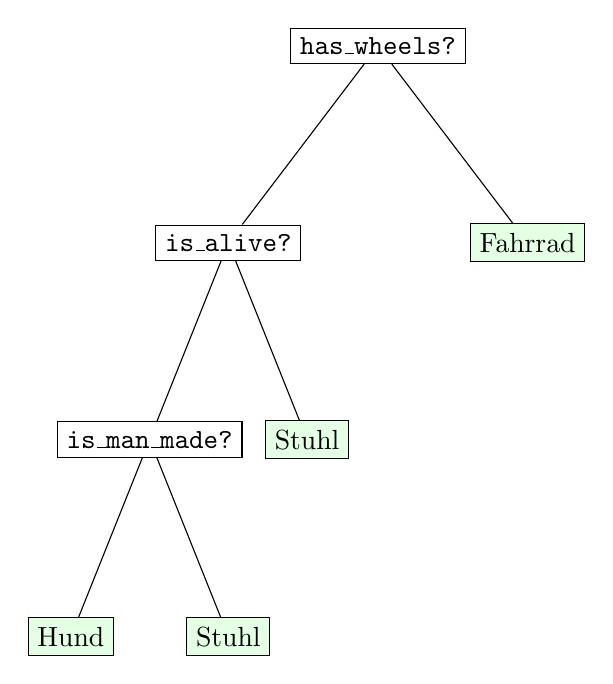
\begin{tikzpicture}
\node[rectangle,draw]{\texttt{has\_wheels?}}
  child {node[rectangle,draw]{\texttt{is\_alive?}}
    child {node[rectangle,draw]{\texttt{is\_man\_made?}}
      child {node[draw,fill=green!10]{Hund}}
      child {node[draw,fill=green!10]{Stuhl}}
    }
    child {node[draw,fill=green!10]{Stuhl}}
  }
  child {node[draw,fill=green!10]{Fahrrad}};
\end{tikzpicture}
\end{aufgabe}

\begin{aufgabe}{IV}
\begin{itemize}
\item Man kann den Baum an echten Beispielen testen und prüfen, wie oft die Vorhersage korrekt ist.
\item Wenn viele Fehler auftreten, sollte man neue, bessere Fragen überlegen oder die Reihenfolge der Fragen anpassen. Auch weitere Daten könnten helfen.
\end{itemize}
\end{aufgabe}